\section{Context asupra sistemului per ansamblu}

Înainte de a discuta de implementarea propriu zisă a proiectului merită să discutăm un pic despre apartanența acestuia într-un sistem mai amplu. Dacă pană acum am descris soluții actuale de pe piață care includeau doar o tablă de șah, un ceas și un anumit sistem de calcul, am lăsat la o parte chestiunea brațului robotic. Într-adevăr în cadrul unei partide împotriva calculatorului (sau a mai multor în paralel) se poate folosi un astfel de braț pentru a deplasa piesele, eliberându-l pe jucătorul uman de această sarcină. \\

Problematica proiectării și dezvoltării brațului fiind în sine o provocare interesantă nu e de mirare faptul ca unul dintre absolvenții Facultății de Inginerie a Universității Lucian Blaga din Sibiu, Pațanghel Cristian-Florian, a implementat așa ceva ca parte a lucrării sale de dizertație \cite{breazu2024robotic}. Brațul robotic elaborat oferă de asemenea utilizatorului o interfață grafică și un protocol serial prin care acesta poate fi controlat prin comenzi de deplasare pe tablă precum \textit{moveToPos(x,y)} sau de gestiune a gripper-ului, \textit{Gripperopen()}.

\begin{figure}[H]
	\centering
	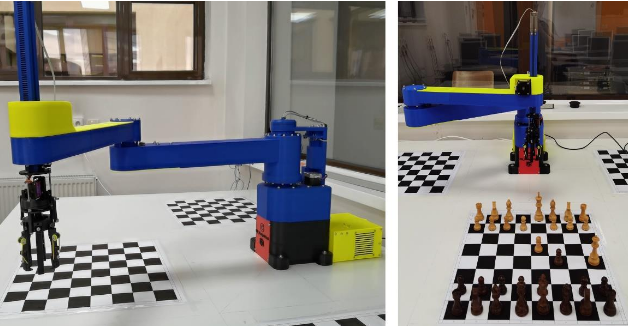
\includegraphics[width=0.7\textwidth]{img/robot_patanghel.png}
	\caption{Brațul robotic aflat în Facultatea de Inginere}
\end{figure}